\documentclass[11pt]{article}
\usepackage{graphicx}
\usepackage{float}

\begin{document}
\title{Lesson 21: Boundary Value Problems}
\author{Colt Bradley}
\date{}
\maketitle

\section{Part 1}

In this first part, we use the relaxation equation defined in the instructions, repeating it until a certain error threshold is allowed between subsequent sweeps. The error threshold is noted in each graph, and in the comment below each graph the number of sweeps it too to meet that threshold is noted. 

Though there is a significant step difference in the last three graphs, they look fairly similar. We need to judge the trade off between having a more exact result and the time it takes to compute that result. If we only need the graph, then perhaps graph (c) would be enough. 

\begin{figure}[H]
\centering
\begin{tabular}{cc}
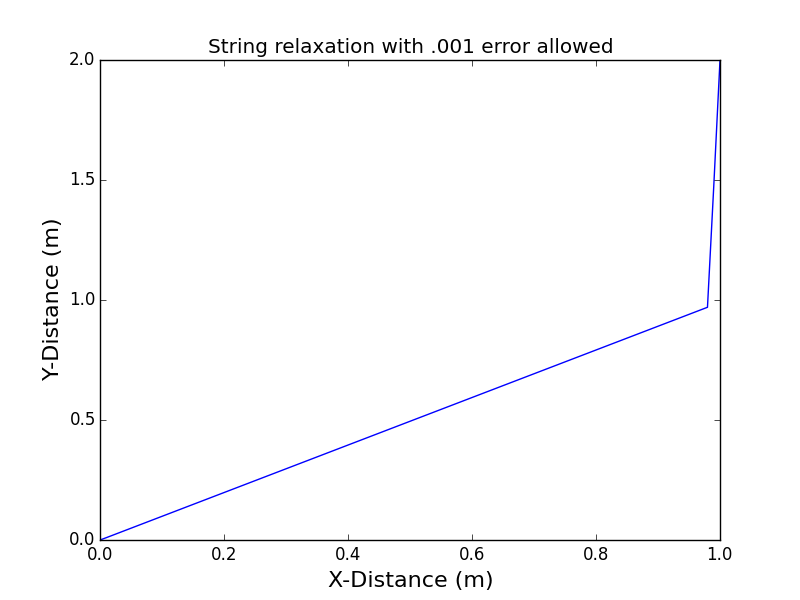
\includegraphics[scale=.3]{1_relaxation(001).png} & 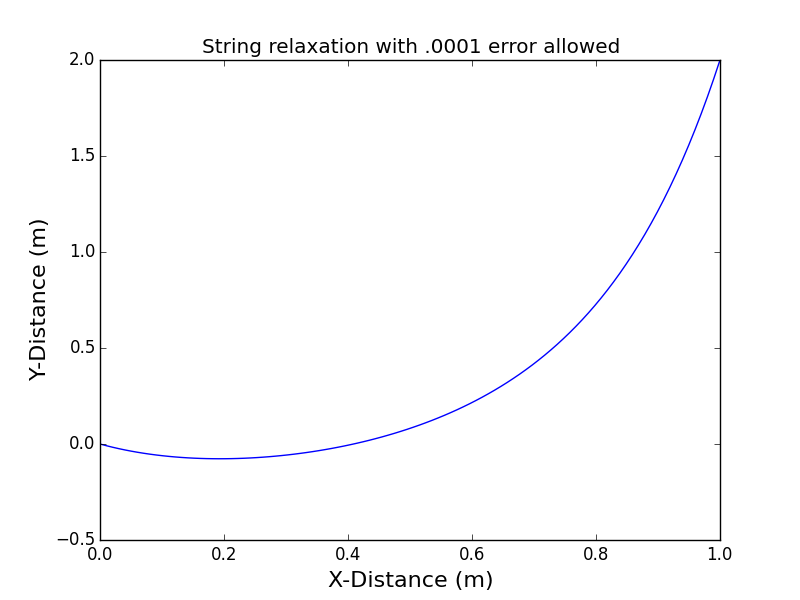
\includegraphics[scale=.3]{1_relaxation(0001).png} \\
(a) After 1 sweep & (b) After 1781 sweeps \\[6pt]


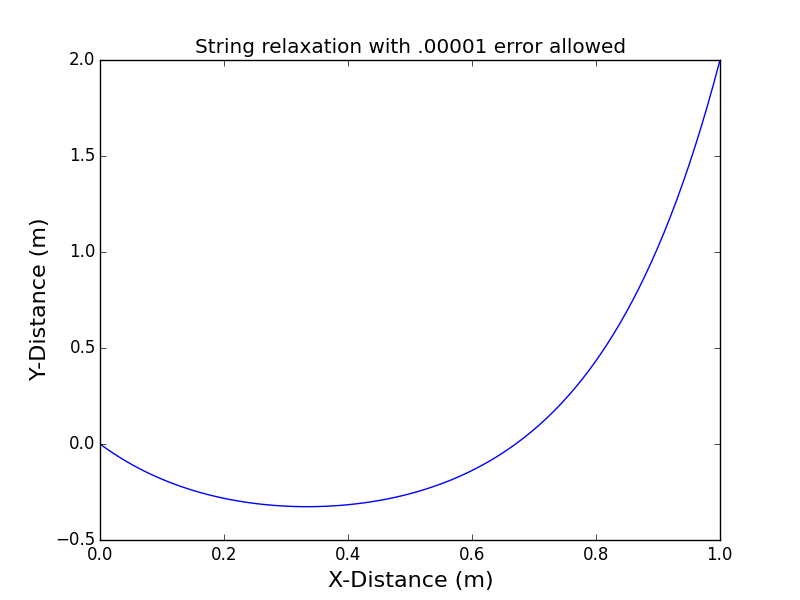
\includegraphics[scale=.3]{1_relaxation(00001).png} & 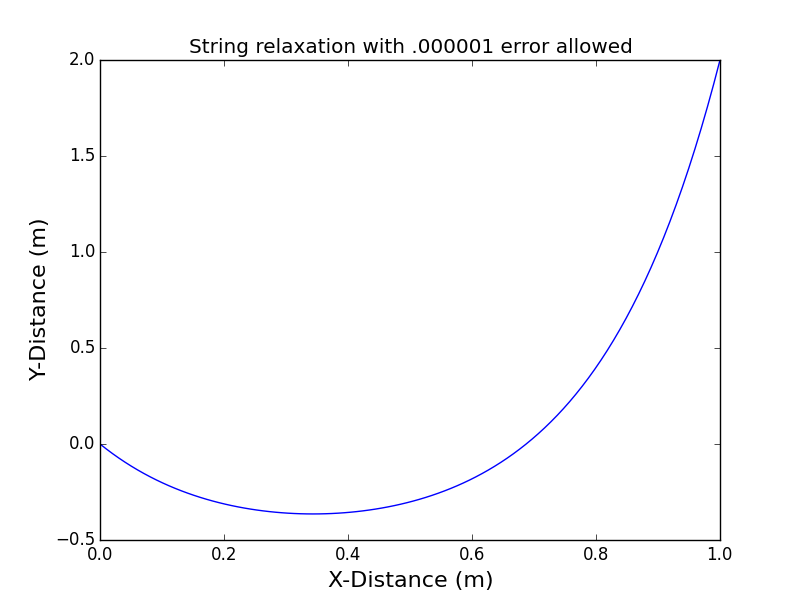
\includegraphics[scale=.3]{1_relaxation(000001).png}\\
(c) After 8709 sweeps & (d) After 16861 sweeps \\[6pt]

\multicolumn{2}{c}{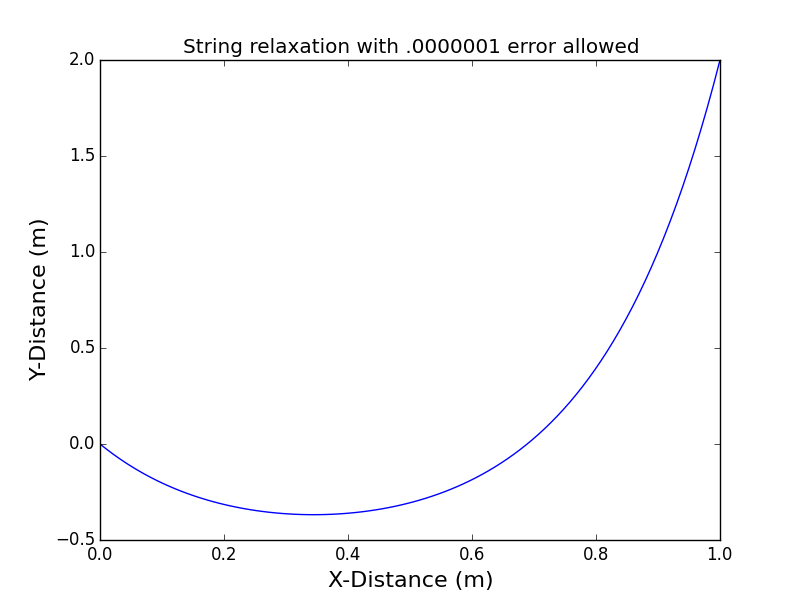
\includegraphics[scale=.3]{1_relaxation(0000001).png}}\\
\multicolumn{2}{c}{(e) After 25139 sweeps} \\[6pt]
\end{tabular}
\caption{Various plots for $\cos (6\pi t) e^{-t^2} $}
\end{figure}

\section{Part 2}
For this section, we try a more sophisticated method of the error threshold in the last part. We use a norm L. I define a function for this, given below, and apply it in a similar way.
 
\begin{verbatim}
def L_1(N,Y):
    sum=0
    for i in range(N+1)[1:-1]:
        sum = sum + (Y[i]-Y[i-1])**2
    return (1./N)*sum
\end{verbatim}

However, we see that we only get to 448 steps, which is short of the roughly 8000 sweeps required to get the graphs in the previous section. When the tolerance of L is decreased any more than the value specified in the title of the graph, the code loops and doesn't output a value. 

\begin{figure}[H]
\centering
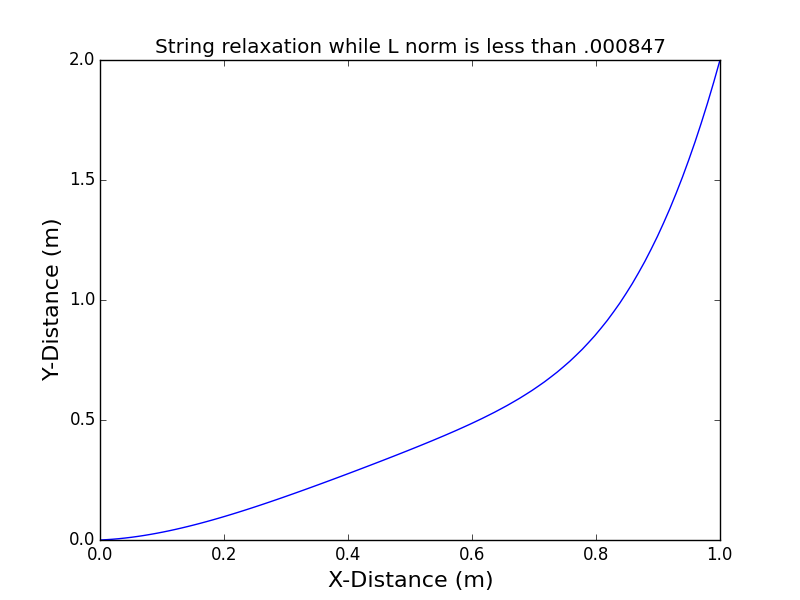
\includegraphics[scale=.4]{2_relaxationWithL.png}
\end{figure}

\section{Part 3}
We know the length of the string is 
\begin{equation}
L = \int_{0}^{1} \sqrt{1+(dy/dx)^2}dx
\end{equation}
where 
\begin{equation}
\frac{dx}{dy}_i = \frac{y_{i+1}-y_{i-1}}{2h}
\end{equation}

The integral can be calculated in the closed form by summing the integrated over all nodes and multiplying by h. This integral is evaluated for various k, and then is plotted against k below. Notice that each is approximately equal to one, as it should be. 

\begin{figure}[H]
\centering
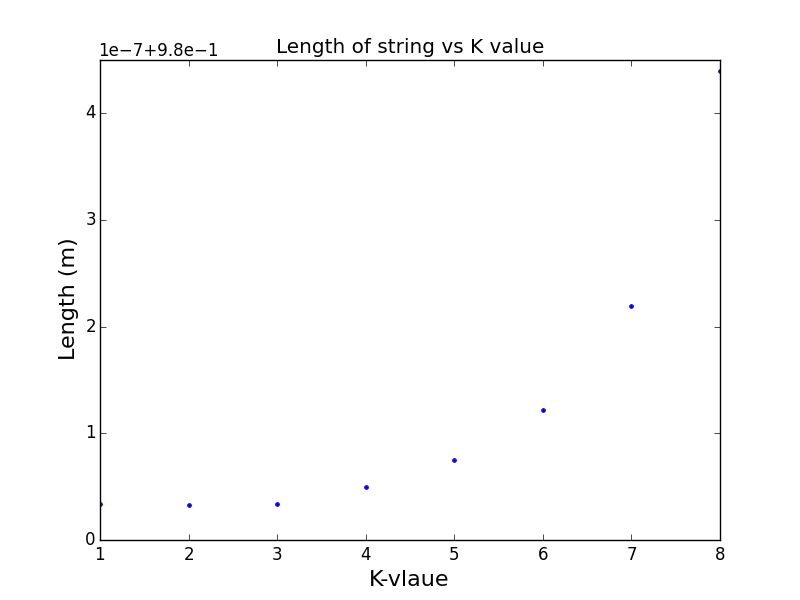
\includegraphics[scale=.4]{3_LvK.png}
\end{figure}
\section{Code}
\subsection{Part 1 Code}
\begin{verbatim}
#Colt Bradley
#4.18.16
#Lesson 21: Boundry Value Problems

###############################################################################
#Import Modules and define functions
###############################################################################
import numpy as np
import pylab as py

###############################################################################
#Part 1
###############################################################################

#define values
k=5.
x_0=0.
x_f=1.
y_0=0.
y_f=2.
N=100.
change = 10.
ch=[]
steps=0
h = (x_f-x_0)/N
X=np.linspace(0,1,100)
#build list of y values
Y=np.zeros(N)
Y[0]=y_0
Y[-1]=y_f
for i in range(len(Y+1))[1:-1]:
    Y[i]=Y[i-1]+h
ch.append(Y[50])

#set the loop to happen while outside a certain error tolerance
while change>.0000001:    
    Y[1:-1] = .5*(Y[:-2]+Y[2:])-(k*h**2)/2.*np.sqrt(1+((Y[:-2]-Y[2:])**2)/(2*h)**2)
    ch.append(Y[50])
    change = abs(ch[-1]-ch[-2])
    steps= steps+1

#print number of sweeps required for the code to run
print steps

py.close()
py.plot(X,Y,"b")
py.title("String relaxation with .0000001 error allowed")
py.xlabel("X-Distance (m)",fontsize = 16)
py.ylabel("Y-Distance (m)",fontsize = 16)
py.savefig("1_relaxation(.0000001).png")
py.show()
\end{verbatim}
\subsection{Part 2 Code}
\begin{verbatim}
#Colt Bradley
#4.18.16
#Lesson 21: Boundry Value Problems

###############################################################################
#Import Modules and define functions
###############################################################################
import numpy as np
import pylab as py

###############################################################################
#Part 2
###############################################################################
#Colt Bradley
#4.18.16
#Lesson 21: Boundry Value Problems

###############################################################################
#Import Modules and define functions
###############################################################################
import numpy as np
import pylab as py

def L_1(N,Y):
    sum=0
    for i in range(N+1)[1:-1]:
        sum = sum + (Y[i]-Y[i-1])**2
    return (1./N)*sum

###############################################################################
#Part 1
###############################################################################

#define values
k=5.
x_0=0.
x_f=1.
y_0=0.
y_f=2.
N=100
L = 10.
ch=[]
steps=0
h = (x_f-x_0)/N
X=np.linspace(0,1,100)
#build list of y values
Y=np.zeros(N)
Y[0]=y_0
Y[-1]=y_f
for i in range(len(Y+1))[1:-1]:
    Y[i]=Y[i-1]+h
ch.append(Y[50])

#set the loop to happen while outside a certain error tolerance
#we'll look at the error tolerance half way through the chain
while L>.000847:    
    Y[1:-1] = .5*(Y[:-2]+Y[2:])-(k*h**2)/2.*np.sqrt(1+((Y[:-2]-Y[2:])**2)/(2*h)**2)
    ch.append(Y[N/2])
    L = L_1(N,Y)
    steps= steps+1

#print number of sweeps required for the code to run
print steps

py.close()
py.plot(X,Y,"b")
py.title("String relaxation while L norm is less than .000847")
py.xlabel("X-Distance (m)",fontsize = 16)
py.ylabel("Y-Distance (m)",fontsize = 16)
py.savefig("2_relaxationWithL.png")
py.show()
\end{verbatim}
\subsection{Part 3 Code}
\begin{verbatim}
#Colt Bradley
#4.18.16
#Lesson 21: Boundry Value Problems

###############################################################################
#Import Modules and define functions
###############################################################################
import numpy as np
import pylab as py

###############################################################################
#Part 2
###############################################################################
#Colt Bradley
#4.18.16
#Lesson 21: Boundry Value Problems

###############################################################################
#Import Modules and define functions
###############################################################################
import numpy as np
import pylab as py

def L_1(N,Y):
    sum=0
    for i in range(N+1)[1:-1]:
        sum = sum + (Y[i]-Y[i-1])**2
    return (1./N)*sum

#fucntion simpson() is the simpson rule function
def simpson(f,a,b,N):
    h = float(b-a)/N
    i = 1
    n = 1
    
    I_1 = 0.
    while i < N:
        I_1 += f(a+i*h)
        i += 1
    
    I_2 = 0   
    while n < N+1:
        I_2 += f(a+n*h - h/2)
        n += 1
    return (h/6)*(f(a)+f(b)+2*I_1+4*I_2)
###############################################################################
#Part 3
###############################################################################

#define values
x_0=0.
x_f=1.
y_0=0.
y_f=2.
N=100
L = 10.
ch=[]
steps=0
h = (x_f-x_0)/N
X=np.linspace(0,1,100)
#build list of y values
Y=np.zeros(N)
Y[0]=y_0
Y[-1]=y_f
for i in range(len(Y+1))[1:-1]:
    Y[i]=Y[i-1]+h
ch.append(Y[50])
R=[]

#set the loop to happen while outside a certain error tolerance
#we'll look at the error tolerance half way through the chain
#we use the open form for the integral
for k in [1.,2.,3.,4.,5.,6.,7.,8.]:
    ch=[]
    for i in range(len(Y+1))[1:-1]:
        Y[i]=Y[i-1]+h
    ch.append(Y[50])
    change = 10    
    while change>.00001:    
        Y[1:-1] = .5*(Y[:-2]+Y[2:])-(k*h**2)/2.*np.sqrt(1+((Y[:-2]-Y[2:])**2)/(2*h)**2)
        ch.append(Y[50])
        change = abs(ch[-1]-ch[-2])
        steps= steps+1
    F=[]
    I=0
    for i in range(100)[1:-1]:
        F.append(np.sqrt(1+((Y[i+1]-Y[i-1])/2*h)**2)*h)
    for k in F[1:-1]:
        I=I+k
    I = I+(3/2)*F[0]+(3/2)*F[-1]
    R.append(I)

py.close()
py.plot([1.,2.,3.,4.,5.,6.,7.,8.],R,"b.")
py.title("Length of string vs K value")
py.xlabel("K-vlaue",fontsize = 16)
py.ylabel("Length (m)",fontsize = 16)
py.savefig("3_LvK.png")
py.show()
\end{verbatim}

\end{document}